\documentclass[diploma]{nanolab2015}

\usepackage{float}
\usepackage{subfigure}
\usepackage{booktabs}
\usepackage{dcolumn}
\usepackage[flushleft]{threeparttable}
\usepackage{makecell}
\usepackage{enumitem}
\usepackage{xparse}
\newcounter{descriptcount}
\NewDocumentEnvironment{enumdescript}{O{}}{%
    \setcounter{descriptcount}{0}%
    \renewcommand*\descriptionlabel[1]{%
      \stepcounter{descriptcount}%
      \normalfont\bfseries ##1%
    }%
    \description%
  }%
  {\enddescription}



\DeclareMathOperator{\Attention}{Attention}
\DeclareMathOperator{\softmax}{softmax}
\DeclareMathOperator{\ReLU}{ReLU}
\DeclareMathOperator{\MSE}{MSE}
\DeclareMathOperator{\AdamW}{AdamW}


\begin{document}
\begin{titlepage}
    \begin{center}
        \large
        Федеральное государственное бюджетное образовательное учреждение
        высшего образования «Московский государственный университет имени
        М.В.Ломоносова»

        МЕХАНИКО-МАТЕМАТИЧЕСКИЙ ФАКУЛЬТЕТ

        \textbf{Кафедра Математической теории интеллектуальных систем}\\
        \vspace{4cm}
        \textsc{\Large Курсовая работа}\\[5mm]
        {\LARGE TODO}
    \end{center}
    \vspace{3cm}
    \null

    \begin{flushright}
        \normalsize \underline{Выполнил:}
        \\студент 431 группы
        \\Зенин В. О.
        \\ \underline{\hspace{4cm}}
    \end{flushright}
    \vspace{1cm}

    \begin{flushright}
        \normalsize \underline{Научный руководитель:}
        \\к.ф.-м.н., н.с Половников В. С.
        \\ \underline{\hspace{4cm}}
    \end{flushright}

    \vfill
    \begin{center}
        \textbf{Москва - 2023}
    \end{center}
\end{titlepage}
\setcounter{page}{3}
\clearpage
\tableofcontents{}  % оглавление
\clearpage
\chapter{Введение}
В настоящее время прогнозирование временных рядов является одной из наиболее актуальных задач в области анализа данных. Это связано с тем, что временные ряды могут отражать различные экономические, социальные и политические процессы, которые необходимо учитывать при принятии решений в различных сферах жизни. Существует множество методов прогнозирования временных рядов, каждый из которых имеет свои преимущества и недостатки.

Существует много временных рядов, связанных с финансами, например, цены различного
рода активов. Также можно найти описание паттернов движения цены, полученные путём анализирования исторических данных биржевых котировок. Многие трейдеры используют их как основание для своих стратегий. Правила, образующиеся в результате найденных закономерностей, достаточно примитивны, как и сами паттерны. Если предположить, что кем-то найдена выгодная стратегия, то подобную способны найти и многие другие участники рынка, сводя на нет любую потенциальную выгоду. Вызывает интерес: способны ли нейронные сети находить паттерны и, тем самым, определять приносящие доход стратегии торговли, скрытые от большинства трейдеров.

Информация о классических финансовых инструментах во многом скрыта и хранится на биржах. Финансовые транзакции также скрыты за межбанковским обменом и не поддаются анализу. Однако существуют набирающие популярность криптофинансовые активы, информация о которых, по своей природе, намного более открыта и может быть использована для анализа движения цены.

Цель данной работы -- исследование доступной публично информации о криптовалютах, построение нескольких архитектур нейронных сетей для анализа исторических данных и построение прогноза изменения будущей цены актива на примере Bitcoin

\newpage
\section{Методы прогнозирования временных рядов}
\subsection{AR(p)}
Одним из методов прогнозирования временных рядов является использование AR (авторегрессионных) моделей \cite{book1}. AR модели позволяют учитывать прошлые значения временного ряда для предсказания его будущих значений. Авторегрессионный процесс задается следующим образом:

$$
    X_t = \beta_0 + \sum_{i=1}^{p}\beta_i X_{t-i} + \varepsilon_t,
$$
где $X_t$ -- будущее значение, которое необходимо предсказать, $\beta_i$ -- параметры модели, $p$ -- порядок модели, независимые одинаково распределенные случайные величины $\varepsilon_t \sim N(0, 1)$.

\subsection{MA(q)}
Также широко распространён метод скользящего среднего (Moving Average, MA). Этот метод основан на усреднении значений временного ряда за определенный период времени. Модель скользящего среднего $q$-го порядка определяется как

$$
    X_t = \sum_{i=0}^{q}\beta_i \varepsilon_{t-i}
$$

\subsection{Exponential Smoothing}
Для усреднения временного ряда кроме скользящего среднего можно использовать экспоненциальное сглаживание. Таким образом получается следующая модель\cite{book2}:

$$
    S_t =
    \begin{cases}
        C_t, t = 1 \\
        C_{t-1} + \alpha \cdot (C_t - S_{t-1}) t > 1
    \end{cases},
$$

где $S_t$ -- сглаженный ряд, $C_t$ -- исходный ряд, $\alpha$ -- коэффициент сглаживания, $\alpha > 0$ и обычно не превосходит $1$ или $2$.

\subsection{Seasonal Decomposition}
Для рядов с выраженной сезонностью существует метод сезонной декомпозиции -- он позволяет выделить сезонные компоненты из общего ряда, что даёт возможность прогнозировать поведение временного ряда в зависимости от сезонных факторов. В данном методе временной ряд делится на две составляющие: сезонную и трендовую. Сезонная составляющая представляет собой повторяющиеся колебания, связанные с сезонными факторами (например, сезонность продаж в розничной торговле). Трендовая составляющая отражает общую тенденцию развития ряда\cite{book3},\cite{book4}.

Описанные ранее классические методы могут применятся как по-отдельности, так и вместе. Из последнего вытекают комбинированные модели ARMA, ARIMA, SARIMA. В качестве параметров необходимо задать факторы, которые будет использовать модель, например: значения временного ряда из прошлого, размер окна скользящего среднего, сдвиг для сезонности (необходимо чтобы заданные факторы находились в одном и том же сезонном промежутке). Коэффициенты при заданных факторах вычисляются по методу наименьших квадратов\cite{book5}.

\subsection{Decision Trees}
Хорошо зарекомендовали себя методы на основе деревьев решений. Одним из преимуществ деревьев решений является их способность обрабатывать большие объемы данных и находить сложные зависимости между признаками и целевым значением. Они также могут быть легко интерпретированы и объяснены, что делает их полезными для задач прогнозирования временных рядов. Например, если имеются данные о продажах товаров в магазине за последние несколько лет, то можно использовать деревья решений для прогнозирования будущих продаж. Мы можем определить признаки, такие как цена товара, сезонность, количество конкурентов в районе и т.д., и использовать их для создания дерева решений. Каждый узел дерева будет принимать решение на основе значения признака, и на выходе получится прогноз будущих продаж.

Для алгоритмов на основе деревьев решений часто используется градиентный бустинг. Данных подход может быть описан следующим образом: построенное дерево имеет некоторую ошибку в своих предсказаниях, при наличии дифференцируемой функции ошибки можно определить поправочные значения, уменьшающие ошибку (градиент) и затем построить новое дерево, цель которого предсказать поправочные значения. Повторяя данную процедуру множество раз строится последовательность деревьев, в которой каждое новое дерево уточняет результат всех предыдущих\cite{book6}.

Деревья решений не имеют представления о временной зависимости между наблюдениями. Чтобы сообщить им эту информацию необходимо закодировать время в признаках. Например, год, месяц, день недели, информация был ли день выходным или праздником -- всё это может быть частью признаков, по которым будет строиться прогноз. Однако целевой признак, например такой как цена актива или величина продаж не должны включаться. В этом основное отличие от классических моделей, которые предсказывают целевую переменную основываясь на её же значениях в исторических данных.

\subsection{Neural Networks}
Также существуют различные подходы на основе нейронных сетей, которые могут использоваться для работы с изменяющимися во времени данными. В процессе своего обучения они способны извлекать сложные нелинейные зависимости из данных и генерировать своё предсказание, основываясь на этом.

В данной работе основное внимание сосредоточено на архитектурах LSTM и Transfomer.

\chapter{Основная часть}
\section{Формальная постановка задачи}
Пусть дан состоящий из $T$ наблюдений временной ряд
$
    X = \{x_t : x_t \in \mathbb{R}^{n+1}\}_{t=1}^T
$.
Выделим из $x_t$ вектор признаков $\vec{x}_t$ и целевое значение $y_t$, таким образом, что
$
    \forall \; t \in \{1, \dotsc, T\} \; \exists \; (\vec{x_t}, y_t)
$,
где $\vec{x}_t \in \mathbb{R}^n $, $y_t \in \mathbb{R}$.
Сформируем пары
$
    (X_{[m;t]}, Y_{t})
$,
где
$
    X_{[m;t]} = \{\vec{x}_{t-m}\}_{j=t-m}^{t-1}
$ -- подпоследовательность фиксированной длины $m$, $Y_t$ -- значение целевого признака.
Для задачи регрессии можно положить $Y_t = y_t$, для задачи классификации
$Y_t \in \{0, \dotsc, K\}$, где $K$ -- количество классов, на которые можно разбить $y_t$.
Требуется построить и оценить качество модели, принимающей на вход последовательность векторов $X_{[m;t]}$ и возвращающей значение $Y_t$.
\section{Данные}
В данной работе использованы дневные наблюдения о состоянии блокчейн сети Bitcoin с 10 мая 2020 года по 8 мая 2023 года, полученные с \href{https://www.blockchain.com/explorer/charts}{blockchain.com}. Некоторые базовые признаки также вычислены заранее поставщиком данных. Их описания собраны в таблице \ref{table:features}.\footnote{Признаки, отмеченные (*) имеют не более 3 пропущенных значений, которые восстановлены линейной интерполяцией.}

\subsection{Предобработка}
При работе с ценой актива часто используется логарифм цены,
$$
    \ln\left(\frac{x_{t}}{x_{t-1}}\right)
$$
позволяющий перейти от абсолютных значений к относительным. Смысл данного преобразования заключается в том, что успешная стратегия приносит доход в результате изменения цен, умноженных на вложенный капитал и именно доход имеет ключевое значение.

Входные данные для нейронных сетей следует скалировать. Однако некоторые признаки в наших данных имеют количественную природу, что выражается в почти линейном росте. Например, абсолютное значение добытых на момент времени $t$ монет BTC. Больший смысл имеет изменение в добыче, так как оно потенциально способно дать сигнал о будущих движениях цены. Поэтому в нашем случае подобное преобразование уместно применить ко всем признакам.

До логарифмирования имелось 1094 векторов, размерности 27 каждый. В результате преобразования наблюдение за первый день вырождается и остается 1093 вектора значений.

\subsection{Формирование обучающего, валидационного и тестового множества}
Для обучения использовались значения до 15 июня 2022 года. Для валидации -- с 15 июня 2022 года по 20 января 2023 года. Для теста -- с 20 января 2023 года по 8 мая 2023 года. Данные временные диапазоны выбраны чтобы обеспечить соотношение 70:20:10.

Целевой признак -- market-price.

Сформируем из данных пары $(X_{[m;t]}, Y_{t})$. $Y_t$ -- значение целевого признака. Пусть $y_t$ -- логарифм цены, выделенный из исходного набора данных и преобразованный в разность логарифмов подряд идущих значений. Тогда становится удобно построить на его основе $Y_t$ для задачи бинарной классификации:
$$
    Y_t =
    \begin{cases}
        1, y_t > 0 \\
        0, y_t \le 0
    \end{cases}
$$

$X_{[m;t]}$ подаётся на вход модели, предсказание которой сравнивается с $Y_{t}$ используя разумную для решаемой задачи функцию потерь. В нашем случае это бинарная кросс-энтропия.

\renewcommand\theadalign{ll}

\begin{table}[ht]
    \centering
    \caption{Признаки из блокчейн сети Bitcoin}
    \label{table:features}
    \begin{threeparttable}
        \begin{tabular}{l|l}
            \thead{\bf Признак}                           & \thead{\bf Описание}                                        \\
            \midrule\midrule
            \texttt{total-bitcoins (*)}                   & \makecell[l]{Количество добытых монет}                      \\
            \texttt{market-price}                         & \makecell[l]{Средняя цена в USD на крупнейших обменниках}   \\
            \texttt{trade-volume}                         & \makecell[l]{Объем обменянных BTC (USD)}                    \\
            \hline
            \texttt{blocks-size}                          & \makecell[l]{Размер сети блокчейна (MB)}                    \\
            \texttt{avg-block-size}                       & \makecell[l]{Средний размер блока (MB)}                     \\
            \texttt{n-transactions-total}                 & \makecell[l]{Количество транзакций}                         \\
            \texttt{n-transactions-per-block}             & \makecell[l]{Среднее число транзакций на блок}              \\
            \texttt{n-payments-per-block}                 & \makecell[l]{Среднее число наград за валидированный блок}   \\
            \texttt{median-confirmation-time}             & \makecell[l]{Медианное время, за которое обработанная       \\ транзакция добавляется к сети}                 \\
            \texttt{avg-confirmation-time}                & \makecell[l]{Среднее время, за которое обработанная         \\ транзакция добавляется к сети}                   \\
            \hline
            \texttt{hash-rate}                            & \makecell[l]{Мощность сети}                                 \\
            \texttt{difficulty}                           & \makecell[l]{Относительная мера сложности сети -- насколько \\ трудно валидировать очередной блок} \\
            \texttt{transaction-fees}                     & \makecell[l]{Выплаченные BTC за валидацию блоков}           \\
            \texttt{transaction-fees-usd}                 & \makecell[l]{Выплаченные USD за валидацию блоков}           \\
            \texttt{fees-usd-per-transaction}             & \makecell[l]{Среднея выплата в USD за                       \\ валидированную транзакцию} \\
            \texttt{cost-per-transaction}                 & \makecell[l]{Общий доход майнеров,                          \\ разделённый на количество транзакций}         \\
            \hline
            \texttt{n-unique-addresses (*)}               & \makecell[l]{Количество уникальных адресов,                 \\ используемых в сети}  \\
            \texttt{n-transactions}                       & \makecell[l]{Количество подтвержённых транзакций за день}   \\
            \texttt{n-payments}                           & \makecell[l]{Количество подтвержённых выплат за день}       \\
            \texttt{output-volume}                        & \makecell[l]{Объем транзакций за день}                      \\
            \texttt{mempool-count}                        & \makecell[l]{Количество неподтверждённых транзакций}        \\
            \texttt{mempool-growth}                       & \makecell[l]{Рост хранилища неподтверждённых транзакций}    \\
            \texttt{mempool-size}                         & \makecell[l]{Размер хранилища неподтверждённых транзакций}  \\
            \texttt{utxo-count (*)}                       & \makecell[l]{Количество монет, доступных для использования  \\ в качестве оплаты за транзакции} \\
            \texttt{n-transactions-excluding-popular}     & \makecell[l]{Количество транзакций,                         \\ за исключением 100 самых популярных адресов} \\
            \texttt{estimated-transaction-volume (*)}     & \makecell[l]{Оценочная стоимость транзакций (BTC)}          \\
            \texttt{estimated-transaction-volume-usd (*)} & \makecell[l]{Оценочная стоимость транзакций (USD)}          \\
            \hline
        \end{tabular}
    \end{threeparttable}
\end{table}

\section{Методы}
\subsection{LSTM}
LSTM (Long Short-Term Memory) - это тип рекуррентной нейронной сети, который используется для обработки последовательных данных, таких как текст, речь и временные ряды. LSTM-сети состоят из ячеек памяти, схема которой представлена на рисунке \ref{pic1}, которые хранят информацию о предыдущих значениях входных данных. Каждая ячейка имеет несколько состояний, которые изменяются в зависимости от входных данных и предыдущих состояний.
Принцип работы LSTM состоит в том, чтобы сохранять информацию о предыдущем состоянии ячейки и использовать эту информацию для принятия решения о текущем состоянии ячейки. Это позволяет LSTM-сетям обрабатывать длинные последовательности данных и учитывать контекст\cite{book8}.

Входной блок принимает на вход данные из предыдущей ячейки и передает их в блок памяти и выходной блок. Блок памяти хранит информацию о предыдущих данных и может использовать эту информацию для прогнозирования следующего значения. Выходной блок вычисляет прогнозное значение на основе информации из блока памяти и входного блока.

\begin{figure}[ht]
    \centering
    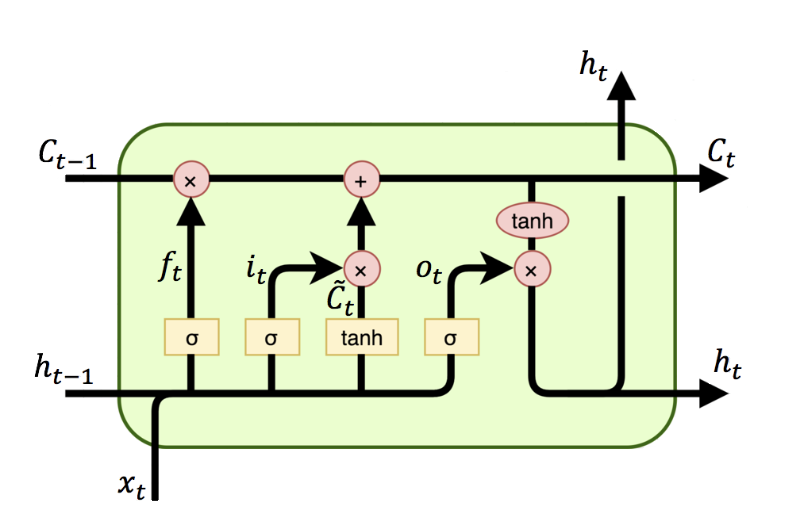
\includegraphics[scale=0.7]{./assets/lstm-cell.png}
    \caption{Схема LSTM-ячейки}
    \label{pic1}
\end{figure}

Формулы для вычисления значений в LSTM ячейке могут быть следующими:
\begin{align*}
    f_t             & = \sigma(W_f \cdot [h_{t-1}, x_t] + b_f)        \\
    i_t             & = \sigma(W_i \cdot [h_{t-1}, x_t] + b_i)        \\
    o_t             & = \sigma(W_o \cdot [h_{t-1}, x_t] + b_o)        \\
    \widetilde{C}_t & = tanh(W_c \cdot [h_{t-1}, x_t] + b_c)          \\
    C_t             & = f_t \cdot C_{t-1} + i_t \cdot \widetilde{C}_t \\
    h_t             & = o_t \cdot tanh(C_t)
\end{align*}
где $i_t$ - вес входного сигнала, $f_t$ - вес забытого сигнала, $o_t$ - вес выходного сигнала, $c_t$ - значение ячейки памяти, $h_t$ - прогнозируемое значение. $W$ - матрица весов ячейки, $b$ вектор сдвига. $W$ в формулах являются различными частями этой матрицы, конкатенация векторов $[\cdot, \cdot]$ позволяет оптимизировать вычисления.

\subsubsection{Bidirectional LSTM}
Bidirectional LSTM - это разновидность рекуррентной нейронной сети, которая также используется для обработки последовательностей данных. Принцип работы этой сети основан на использовании двух LSTM-слоев: прямого и обратного.
Прямой LSTM слой обрабатывает последовательность с начала до конца, а обратный LSTM слой - в обратном порядке. Затем результаты от обоих слоев объединяются, чтобы получить более точную оценку для каждого элемента последовательности\cite{book9}.

\begin{figure}[ht]
    \centering
    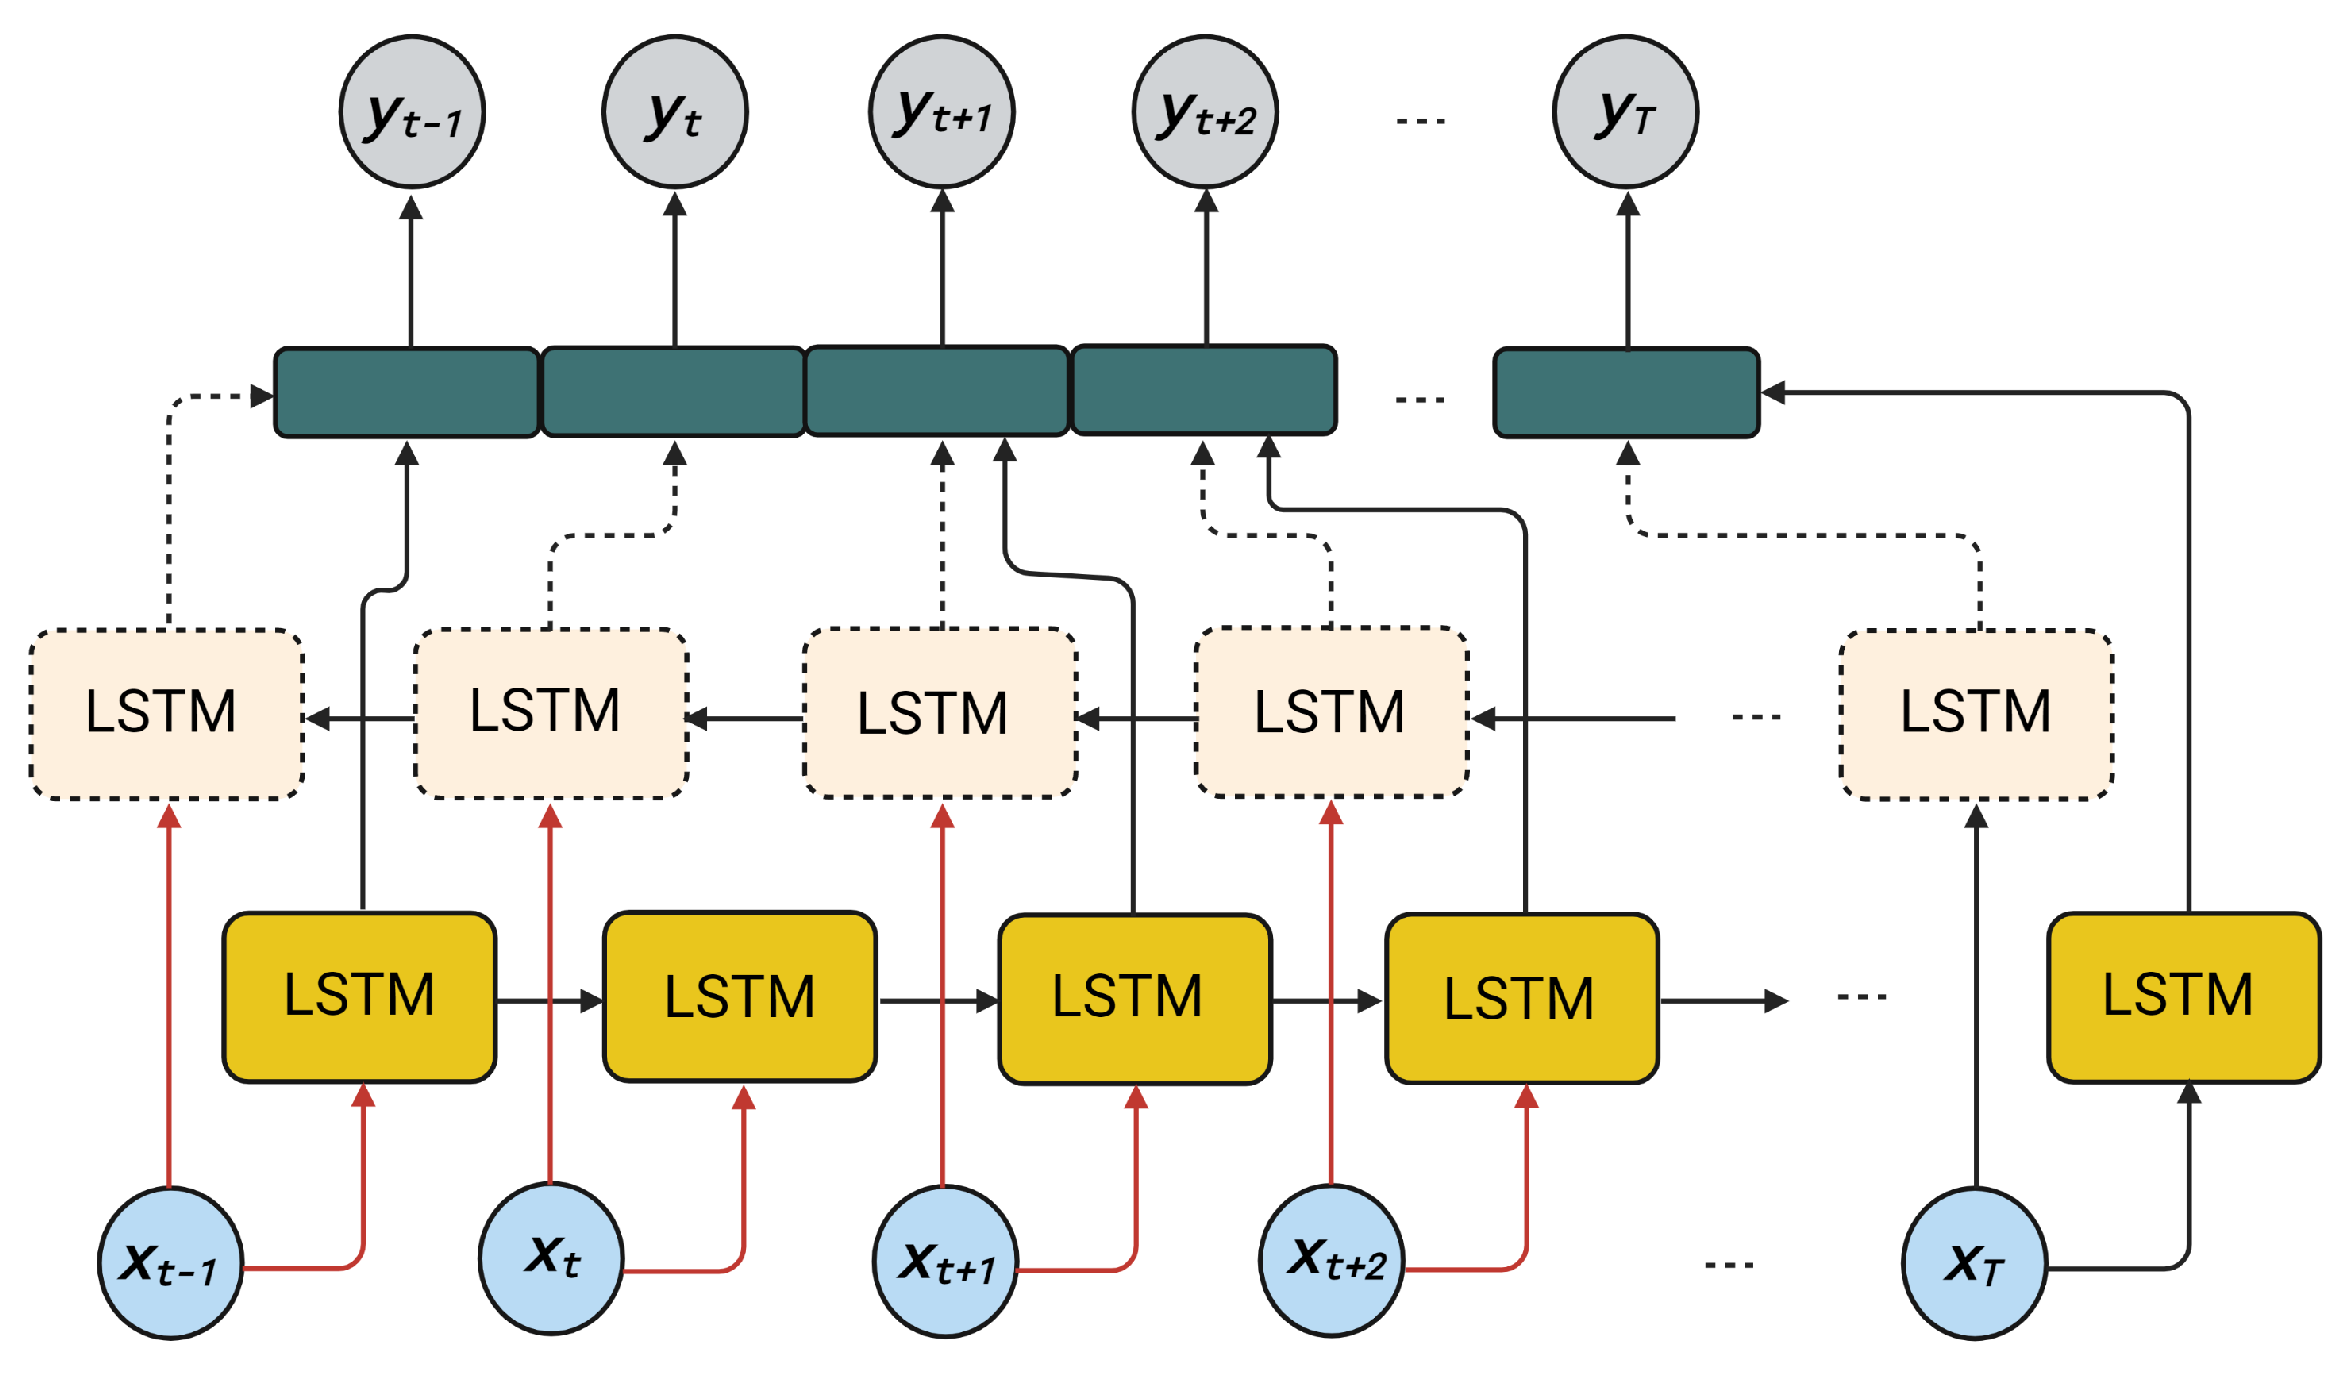
\includegraphics[scale=0.2]{./assets/lstm-bidirectional.png}
    \caption{Схема двунаправленной рекуррентной сети на основе ячейки LSTM}
    \label{pic2}
\end{figure}

\subsection{Transformer}
% TODO: Описать подробнее про трансформер с картинкой в виде двух блоков

\subsubsection{Self-attention}
Модель извлекает из входных данных информацию при помощи механизма внутреннего внимания (self-attention) и использует ее для формирования выходных данных.

\begin{figure}[ht]
    \centering
    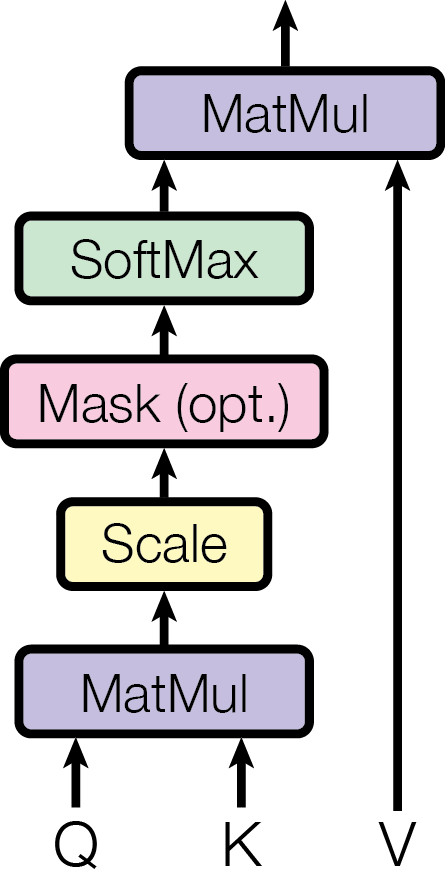
\includegraphics[scale=0.2]{./assets/self-attention.png}
    \caption{Scaled Dot-Product Attention\cite{book10}}
    \label{pic3}
\end{figure}

Пусть в качестве функции внимания используется скалярное произведение
$$
    \vec{q} \cdot \vec{k} = \sum_{i=1}^{d_k}q_i k_i
$$
Обозначим за $Q = K = V$ матрицы, в строках которых записаны векторы входной последовательности, каждый вектор имеет размерность $d_k$.
Тогда принцип работы self-attention можно описать следующим образом:
\begin{enumerate}
    \item Создание матрицы внимания: Матрица внимания представляет собой квадратную матрицу размерности $N$, где $N$ - количество элементов входной последовательности.Для её создания необходимо вычислить скалярное произведение между каждым элементом входного вектора и всеми остальными элементами $$QK^\top$$
    \item Нормализация: Сумма всех значений в каждом столбце матрицы внимания должна быть равна 1, чтобы сохранить сумму всех значений в данных неизменной. Это достигается путем нормализации матрицы внимания с использованием softmax функции. Также перед применением softmax имеет смысл поделить все значения матрицы на $\sqrt{d_k}$. Это помогает компенсировать негативный эффект от проклятия размерности. $$\softmax(\frac{QK^\top}{\sqrt{d_k}})$$
    \item Умножение на веса: Каждый элемент матрицы представляет собой вес, в некоторой мере отражающий схожесть между векторами входной последовательности. Теперь необходимо вычислить взвешенную сумму $$\softmax(\frac{QK^\top}{\sqrt{d_k}}) \cdot V$$
\end{enumerate}

\subsubsection{Multi-Head Attention}
Возможности данной операции расширяются использованием механизма множественного внимания, который, в свою очередь, позволяет модели применить внутреннее внимание несколько раз на разные части входной последовательности, тем самым получая возможность извлечь больше полезной информации. Реализуется это следующим образом:
\begin{enumerate}
    \item Входные данные проецируются в векторы меньшей размерности независимыми линейными слоями.
    \item Каждый полученный вектор проходит через свой self-attention. Данная часть называется `головой' (head).
    \item Результирующие векторы объединяются путём конкатенации.
\end{enumerate}
В общем случае размерности векторов после проекции должны быть равными, то есть изначальная размерность вектора признаков должна быть кратна количеству голов $h$.

\begin{figure}[ht]
    \centering
    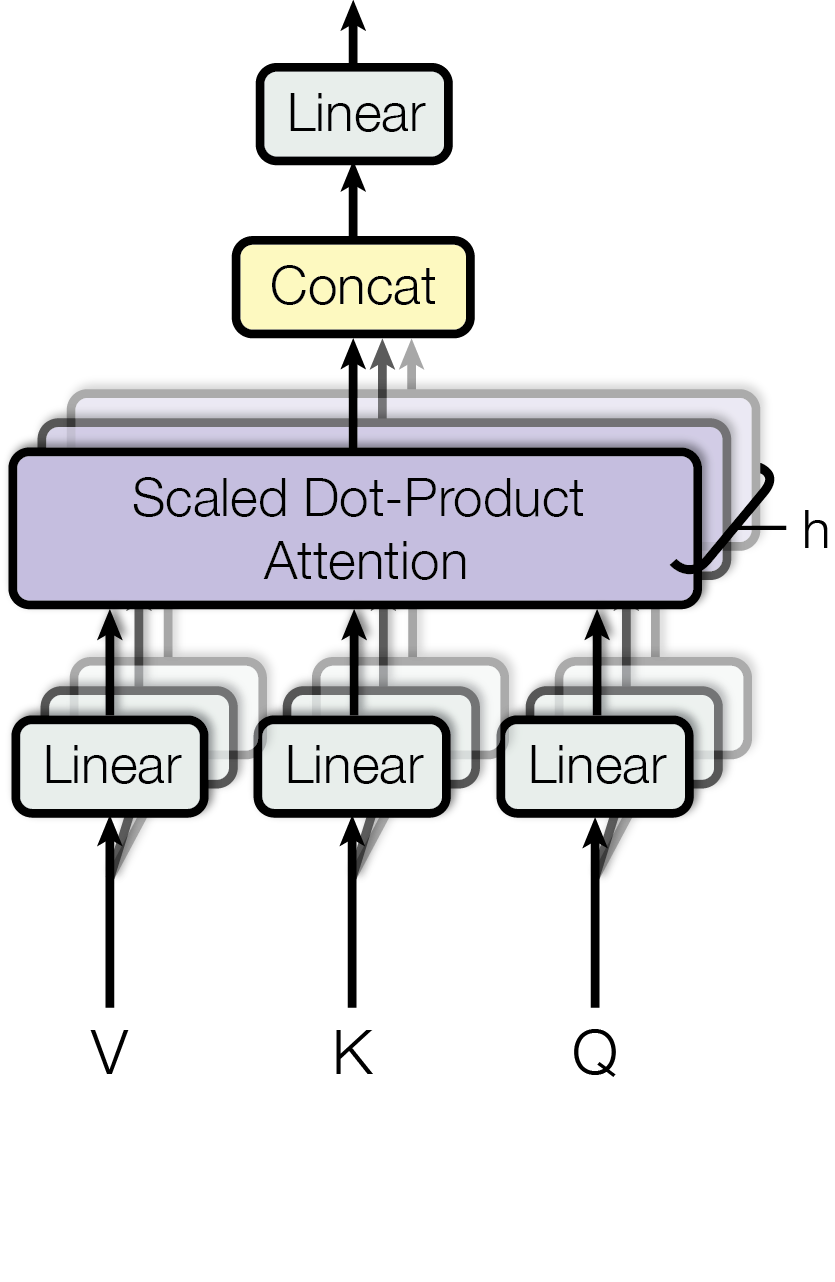
\includegraphics[scale=0.2]{./assets/multi-head-self-attention.png}
    \caption{Multi-Head attention\cite{book10}}
    \label{pic4}
\end{figure}

\subsubsection{Fully-Connected Layer}
Полученный после прохождения блока множественного внимания вектор поступает на полносвязный слой размерности $d_{hid}$ с функцией активации $ReLU$. После чего процедура может повторяться многократно, образуя слои энкодера. Результирующий вектор может быть использован для решения различных задач.

\subsubsection{Positional Encoding}
Описанная архитектура никак не использует информацию о последовательности подаваемых на вход векторов. В таких задачах как обработка текста или временного ряда необходимо сообщить информацию о позиционной или временной зависимости в данных. Это можно сделать используя следующее преобразование
$$PE_{(pos,2i)} = sin(pos/10000^{2i/d_{model}})$$
$$PE_{(pos,2i+1)} = cos(pos/10000^{2i/d_{model}})$$
$d_{model}$ -- размерность входных данных, с которой работает трансформер. Часто чтобы обеспечить её достаточно отобразить линейным слоем настоящие векторы и получить их эмбеддинги соответствующей размерности. Тогда компоненты $PE_{(pos)}$ прибавляются к компонентам входных векторов $x_{pos}$.

\subsubsection{Encoder-only Transformer}
Encoder-only Transformer (EOT) - это разновидность Transformer, который использует только блок энкодера для генерации выходных данных. Поскольку модель не имеет декодера, ее задача заключается только в преобразовании входных данных в выходные, а не в авторегрессионном генерировании выходной последовательности.


\newpage
\section{Эксперимент}
Решая задачу бинарной классификации в данной задаче удобно использовать ``жёсткий'' подход. Пусть выход модели это двумерный вектор, значения которого преобразованы при помощи $\softmax$:

Тогда каждая компонента говорит о некоторой доле вероятности принадлежности к классу, равному индексу этой компоненты. Данное представление более универсально и позволяет использовать обычную кросс-энтропию, вместо бинарной и не подбирать пороговое значение, которое будет отделять позитивный класс (1, цена пойдёт вверх) от негативного (0, цена пойдет вниз).

Для LSTM не составляет труда получить такое предсказание: можно взять выход последней ячейки, сравнить с ground truth и сделать шаг в изменении весов. Transformer же вернёт последовательность векторов, равную по длине входной последовательности. Для приведения такого выхода к нужному вектору использовался следующий подход:

\begin{enumerate}
    \item Значения векторов последовательности усредняются, в результате чего получается один вектор размерности \texttt{d\char`_model}.
    \item При помощи линейного слоя он отображается в вектор размерности 2
    \item К нему применяется $\softmax$ и вычисляется кросс-энтропия
\end{enumerate}

\subsection{Параметры}
В качестве гиперпараметров, не связанных с архитектруными особенностями моделей были взяты:
\begin{itemize}
    \item \texttt{batch\char`_size}: количество элементов в пакете, который используется для обучения нейронной сети. При обучении с использованием градиентного спуска каждый пакет используется для вычисления градиента ошибки и обновления весов сети. Чем больше размер пакета, тем больше данных используется для вычисления градиента, что может ускорить процесс обучения. Однако, слишком большой размер пакета может привести к переобучению сети и ухудшению ее производительности. Поэтому, выбор оптимального размера пакета является важной задачей при обучении нейронных сетей.
    \item \texttt{max\char`_epoch}: количество проходов всех обучающих данных через модель. Каждая эпоха состоит из обучения на всех данных, а затем проверки производительности модели на тестовом наборе. Количество эпох обычно определяется размером набора данных: чем больше данных, тем больше эпох может потребоваться для обучения.
    \item \texttt{sequence\char`_length}: количество элементов в последовательности, которая используется для обучения нейронной сети. Длина последовательности может влиять на производительность нейронной сети, так как она определяет количество информации, которую сеть может использовать для обучения и прогнозирования. Чем длиннее последовательность, тем больше информации можно использовать для обучения. Однако, слишком длинная последовательность также может привести к переобучению, что может ухудшить производительность модели.
\end{itemize}

\subsubsection{LSTM}
\begin{itemize}
    \item \texttt{num\char`_layers}: количество блоков памяти в каждом слое модели LSTM, а также количество слоев в целом. Чем больше число слоев, тем больше информации может быть сохранено в блоках памяти и использовано при прогнозировании. Однако увеличение числа слоев может привести к увеличению сложности модели и времени обучения.
    \item \texttt{d\char`_hid}: размерность скрытого слоя, т.е. размерность вектора, который представляет состояние ячейки LSTM. Размерность скрытого слоя оказывает значительное влияние на производительность и качество модели. Слишком маленький размер скрытого слоя может привести к недостаточной емкости для хранения информации о предыдущих состояниях ячейки, что может привести к потере информации при обучении модели. Слишком большой размер скрытого слоя также может привести к переобучению модели и снижению ее производительности.
    \item dropout: доля случайно отбрасываемых нейронов в соответствующем методе регуляризации, который используется для предотвращения переобучения.
\end{itemize}

Поскольку используется двунаправленная сеть, то \texttt{d\char`_hid} на самом деле умножается на 2: одна половина используется для прямого прохода, другая для обратного.

\subsubsection{Transformer}
\begin{itemize}
    \item \texttt{num\char`_layers}: количество слоёв, содержащих блок множественного внимания и полносвязный слой с функцией активации $\ReLU$.
    \item \texttt{d\char`_hid}: размерность скрытого слоя, следующего после множественного внимания.
    \item \texttt{d\char`_model}: размерность входных данных, с которой работает Transformer. Она может быть не равна количеству признаков в используемом датасете, поэтому требует линейного преобразования.
    \item \texttt{n\char`_head}: число голов блока множественного внимания.
    \item dropout: используется после скрытого слоя.
\end{itemize}

\subsubsection{Подбор параметров}
LSTM из-за своих архитектурных особенностей позволяет выбрать любые параметры независимо. Transformer же требует, чтобы, например, \texttt{n\char`_head} делило \texttt{d\char`_model}. Поэтому для перебора были выбраны различные степени двойки, чтобы обеспечить делимость для любого набора выбранных параметров. Диапазоны и финальные параметры, на которых выполнялось тестирование, описаны в таблице \ref{table:hyperparam_lstm} для LSTM и в таблице \ref{table:hyperparam_transformer} для Transformer.

Параметры перебирались при помощи фреймворка \href{https://optuna.org/}{optuna} в заданных диапазонах. В качестве метрики для сравнения моделей с различными параметрами использовалась точность (Accuracy). Заведомо неудачные наборы параметров отсекались при помощи MedianPruner: данный метод прерывает обучение, если модель с выбранными параметрами на данном шаге хуже чем медианное значение ранее обученных моделей на этом же шаге.

Для LSTM было взято 400 попыток перебора, для Transformer сначала 400, а затем ещё 200 для более легковесной архитектуры.

Наиболее перспективные результаты для LSTM получались при использовании малых размерностей скрытого слоя и большего числа слоёв LSTM, из чего был сделан вывод что стоит выбрать параметры, указанные в таблице \ref{table:hyperparam_lstm}, но увеличить продолжительность обучения до 500 эпох, поскольку значение функции ошибки на валидации указывало на устойчивость к переобучению.

Transformer давал плохие результаты на первых 400 попытках, говорящие о явном переобучении. Стоило рассмотреть архитектуру с малым числом параметров и повторить перебор. В результате перспективными были определены параметры, указанные как итоговые в таблице \ref{table:hyperparam_transformer}. Также значения функции ошибки на валидации указывали на то, что удалось добиться устойчивости к переобучению и отказаться от метода раннего останова.

% Стоит сделать замечание насчет значений функции ошибки. Поскольку в эксперименте был важен качественный результат, для определения которого не использовалась мера уверенности модели в своем решении, то сравнивать кросс-энтропию между моделями нерелевантно. Основную роль играет тенденция, заключающаяся в росте точности при неувеличении функции ошибки на валидации. Особенно это заметно в обучении модели на базе архитектуры трансформера, для которой лучшие результаты получаются при использовании большого количества данных и эпох обучения. 

С лучшими параметрами на валидации модели были обучены на всех данных, кроме тестовых.

\begin{table}[ht]
    \centering
    \caption{Диапазоны перебора параметров}
    \label{table:hyperparam}
    \begin{minipage}[t]{.5\textwidth}
        \caption{LSTM}
        \label{table:hyperparam_lstm}
        \centering
        \begin{tabular}{l|l|l}
            \thead{\bf Параметр}           & \thead{\bf Диапазон} & \thead{\bf Итог} \\
            \midrule\midrule
            \texttt{batch\char`_size}      & [16, 128]            & 32               \\
            \texttt{max\char`_epoch}       & [5, 2000]            & 500              \\
            \texttt{sequence\char`_length} & [5, 96]              & 40               \\
            \hline
            \texttt{num\char`_layers}      & [2, 12]              & 6                \\
            \texttt{d\char`_hid}           & [16, 256]            & 28               \\
            \texttt{dropout}               & [0.2, 0.5]           & 0.27
        \end{tabular}
    \end{minipage}%
    \begin{minipage}[t]{.5\textwidth}
        \centering
        \caption{Transformer}
        \label{table:hyperparam_transformer}
        \begin{tabular}{l|l|l}
            \thead{\bf Параметр}           & \thead{\bf Диапазон } & \thead{\bf Итог} \\
            \midrule\midrule
            \texttt{batch\char`_size}      & $2^{[4, 7]}$          &                  \\
            \texttt{max\char`_epoch}       & [5, 4000]             &                  \\
            \texttt{sequence\char`_length} & [5, 96]               &                  \\
            \hline
            \texttt{num\char`_layers}      & $2^{[2, 6]}$          &                  \\
            \texttt{dropout}               & [0.2, 0.5]            &                  \\
            \hline
            \texttt{d\char`_hid}           & $2^{[1, 10]}$         &                  \\
            \texttt{d\char`_model}         & $2^{[3, 9]}$          &                  \\
            \texttt{n\char`_head}          & $2^{[0, 3]}$          &
        \end{tabular}
    \end{minipage}
\end{table}


\subsection{Результаты}
Значения на тестовом множестве для моделей перечислены в таблице \ref{table:reults_final}.

\begin{table}[!b]
    \centering
    \caption{Качество на тестовом множестве}
    \label{table:reults_final}
    \begin{threeparttable}
        \begin{tabular}{l|l|l}
            \thead{\bf Метрика} & \thead{\bf LSTM } & \thead{\bf Transformer } \\
            \midrule\midrule
            \texttt{Accuracy}   &                   &                          \\
            \texttt{Precision}  &                   &                          \\
            \texttt{Recall}     &                   &                          \\
            \texttt{F1-Score}   &                   &                          \\
        \end{tabular}
    \end{threeparttable}
\end{table}

\newpage
\begin{thebibliography}{00}
    % \addcontentsline{toc}{section}{Список литературы}
    \bibitem{book1}
    James D. Hamilton. Time Series Analysis and Forecasting. Princeton University Press, 1994.
    \bibitem{book2}
    Everette S. Gardner. Exponential smoothing: The state of the art. 01 Jan 1985-Journal of Forecasting (John Wiley \& Sons, Ltd.)-Vol. 4, Iss: 1, pp 1-28
    \bibitem{book3}
    Lovell, Michael C. Seasonal Adjustment of Economic Time Series and Multiple Regression Analysis. Journal of the American Statistical Association, vol. 58, no. 304, 1963, pp. 993-1010.
    \bibitem{book4}
    Robert Alan Yaffee, Monnie McGee. Introduction to Time Series Analysis and Forecasting: With Applications of SAS and SPSS. Academic press, 2000
    \bibitem{book5}
    Hyndman, R.J., \& Athanasopoulos, G. (2021) Forecasting: principles and practice, 3rd edition, OTexts: Melbourne, Australia.
    \bibitem{book6}
    Panarese, A.; Settanni, G.; Vitti, V.; Galiano, A. Developing and Preliminary Testing of a Machine Learning-Based Platform for Sales Forecasting Using a Gradient Boosting Approach. Appl. Sci. 2022, 12, 11054.
    \bibitem{book7}
    U Thissen, R van Brakel, A.P de Weijer, W.J Melssen, L.M.C Buydens. Using support vector machines for time series prediction. Chemometrics and Intelligent Laboratory Systems, Vol. 69, Iss: 1-2, 2003, pp 35-49.
    \bibitem{book8}
    Sepp Hochreiter and Jürgen Schmidhuber. 1997. Long Short-Term Memory. Neural Comput. 9, 8 (November 15, 1997), 1735-1780.
    \bibitem{book9}
    Schuster, Mike \& Paliwal, Kuldip. (1997). Bidirectional recurrent neural networks. Signal Processing, IEEE Transactions on. 45. 2673 - 2681.
    \bibitem{book10}
    Ashish Vaswani, Noam Shazeer, Niki Parmar, Jakob Uszkoreit, Llion Jones, Aidan N Gomez, Łukasz Kaiser, and Illia Polosukhin. Attention is all you need. In NeurIPS, 2017.
\end{thebibliography}

\end{document}
